\section{Hard X-Ray spectroscopy}
\subsection{Runaway electrons}
The plasma in a tokamak is heated to a level where particles reach a velocity
enabling them to break through atomic repulsion. In such conditions some 
particles can also obtain sufficient speed to escape the magnetic confinement
of the vessel. Typically collisions with other particles are so frequent
that in stable plasma REs are not emitted in large quantities.
Directly after plasma is disrupted or terminated, this probability is 
lessened and a tokamak might start acting like a particle accelerator,
bringing the electrons to nearly the speed of light.
Electrons that act in this manner are called Runaway Electrons (REs).
\cite{iter_re_melt}

This phenomenon can occur in the form of a high-energy 
concentrated beam capable of melting the front-facing walls of a reactor.
The effects of such damage being purposefully introduced in the JET tokamak
are shown in \autoref{fig:re_melt}. To prevent mitigate the destructive
effects of REs their generation has to be avoided if possible. Otherwise
they must be detected and dealt with accordingly. One method of doing so 
involves the injection of noble gases in a process called 
Massive Gas Injection (MGI) \cite{massive_gas_injection}.
 
\begin{figure}
  \centering
  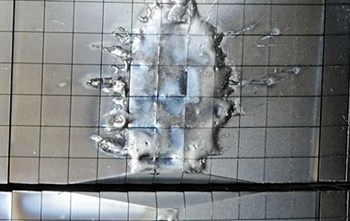
\includegraphics[width=.7\linewidth]{media/re_melt.jpeg}
  \caption{Effects of RE in JET vessel\cite{iter_re_melt}}
  \label{fig:re_melt}
\end{figure}

When REs interact with the Plasma Facing Components (PFCs)
they lose their energy and emit X-Ray radiation in 
the Bremsstrahlung process. The energy of this radiation
varies greatly, ranging from tens of keV (Soft X-Ray)
to multiple MeV (Hard X-Ray).
\cite{hxrm_jet}


\subsection{PhotoMultiplier Tubes}
\subsection{Preamplifiers}
\subsection{Analogue processing chains}
\subsection{Digital processing chains}
